\documentclass[10pt]{beamer}

\usepackage[utf8]{inputenc}
\usepackage{ngerman}
\usepackage[ngerman]{babel}
\usepackage{amsmath}
\usepackage{bbm}

\usepackage{tabularx}
\usepackage{graphicx}
\usepackage{subfigure}
\usepackage{url}
\usepackage{eurosym}
\usepackage{listings}

\usepackage{multirow}
\usepackage{colortbl}
\usepackage{booktabs}
\usepackage{setspace}

\newif\ifzihbackground
\zihbackgroundtrue
%\zihbackgroundfalse

% Yes, this is dirty
\newcommand\zihmaketitle{
	\definecolor{white}{gray}{1.00}%
	\setbeamercolor{normaltext}{bg=darkblue}%
	\setbeamertemplate{headline}{%
		\vskip6.15mm\color{white}\setlength{\arrayrulewidth}{0.3pt}%
		\begin{tabular*}{\paperwidth}[b]{l@{\extracolsep\fill}}%
			\hspace*{3.0mm}\color{white}%
			\includegraphics[height=7.81mm]{theme/logo/tu_logo_black}\\[1.2mm]%
			\hline\hspace*{11.76mm}\rule[-0.8mm]{0pt}{2.47mm}%
			\def\@@dummyComma{}\rule{0pt}{5.8pt}%
			\insertinstitute \\%
			\hline%
		\end{tabular*}%
		\hspace{-\paperwidth}%
	}%
    \ifzihbackground
      \setbeamertemplate{footline}{}
      \setbeamertemplate{background}{
\includegraphics[height=\paperheight,width=\paperwidth]{theme/logo/bg}}
      \else
      \setbeamertemplate{footline}{
          \parbox[t][22mm]{\paperwidth}{
              \vspace*{-8.18mm}
              \rule
              {98.6mm}{0pt}\includegraphics[height=15mm]{theme/logo/zih_logo_white}

          }
      }
    \fi%
   \frame{\titlepage}
    % Kopf-/Fusszeilen fuer restliche Folien
    \setbeamercolor{normal text}{bg=white}
    \setbeamertemplate{background}{}
    \setbeamertemplate{headline}[zih01 theme]
    \setbeamertemplate{footline}[zih01 theme]
}

\usetheme{Dresden}
%\useoutertheme{theme/zih01}
%\useinnertheme{theme/zih01}
\usepackage{theme/beamerouterthemezih01}
\usepackage{theme/beamerinnerthemezih01}

%\useinnertheme{rounded}
\definecolor{darkblue}{rgb}{0.04, 0.16, 0.32}
% font color for headlines etc.
\setbeamercolor*{structure}{fg=darkblue,bg=white}
% disable navigation symbols
\setbeamertemplate{navigation symbols}{}
% can't remember what this is good for
\setbeamercovered{transparent}

% reduce margin size
\setbeamersize{text margin left=0.7cm}
\setbeamersize{text margin right=0.7cm}
%
% Outer Color Theme "whale" sorgt f?r strenge farbliche Trennen zwischen Zierrat
% und dem eigentlichen Inhalt. Ein dunkler Hintergrund f?r den Folientitel wirkt
% aber zu aufdringlich.
%
\usecolortheme{orchid}
%\setbeamercolor{titlelike}{parent=structure}

%
% Inner Color Theme "orchid" sorgt f?r farblich abgesetzt Bl?cke (Definitionen,
% S?tze, Beispiele, Beweise, ...).
%
%\usecolortheme{orchid}

%zum drucken
%\usepackage{pgfpages}
%\pgfpagesuselayout{resize to}[a4paper,border shrink=5mm,port]
%\pgfpagesuselayout{4 on 1}[a4paper,border shrink=3mm, landscape]

%%%%%%%%%%%%%%%%%%%%%%%%%%%%

\definecolor{LightGray}		{gray}{0.9}
\definecolor{Gray}		{gray}{0.5}
\definecolor{DarkGray}     	{gray}{0.2}
\definecolor{listinggray} 	{gray}{0.96}
\definecolor{DarkGreen}     	{rgb}{0.0,0.6,0.0}
\definecolor{DarkRed}     	{rgb}{0.6,0.0,0.0}
\definecolor{DarkBlue}     	{rgb}{0.0,0.0,0.6}
\definecolor{DarkCyan}     	{rgb}{0.7,0.7,0.2}
\definecolor{DarkDarkGreen}	{rgb}{0.0,0.4,0.0}

\lstset{language=C}
\lstset{linewidth=0.99\textwidth}
%\lstset{boxpos=c}
\lstset{xleftmargin=0.03\textwidth}
%\lstset{breaklines=true}
\lstset{framexleftmargin=0.03\textwidth}
\lstset{abovecaptionskip=\smallskipamount}
\lstset{belowcaptionskip=\smallskipamount}
\lstset{basicstyle=\ttfamily\tiny}
\lstset{backgroundcolor=\color{listinggray}}
%\lstset{frameround=ffff}
%\lstset{frame=shadowbox}
%\lstset{rulesepcolor=\color{Gray}}
\lstset{numbers=left}
\lstset{numberstyle=\tiny \color{DarkGray}}
\lstset{numbersep=0.01\textwidth}
\lstset{showstringspaces=false}
%\lstset{showspaces=false}
\lstset{tabsize=4}

%% all words in the following list are printed in bold letters in a listing 
\lstset{emph={__asm__, __volatile__, return, main,},emphstyle={\bfseries\color{DarkGray}}}
\lstset{captionpos=b}

% Style für C Sourcecode
\lstdefinestyle{CA}{
        language=C,
        basicstyle=\ttfamily\scriptsize,
        keywordstyle=\ttfamily\bfseries\color{DarkBlue},
        stringstyle=\ttfamily\color{DarkRed},
        commentstyle=\ttfamily\color{DarkGreen},
        identifierstyle=\ttfamily\color{DarkCyan},
        backgroundcolor=\color{listinggray},
}

%%%%%%%%%%%%%%%%%%%%%%%%%%%%

\title{Escalator}
\subtitle{Flexible On-Call Benachrichtigung}
\author{Hermann Loose}
\email{hermannloose@gmail.com}
\institute[ZIH TUD]{Zentrum für Informationsdienste und Hochleistungsrechnen — TU Dresden}
\date{10. Februar 2012}

\begin{document}

\zihmaketitle
%\frame{\titlepage}

\begin{frame}
  \frametitle{Motivation}
  \begin{flushleft}
    \emph{„do one thing and do it well“} — Douglas McIlroy
  \end{flushleft}
  \begin{itemize}
    \item automatische Eskalation von Ereignissen
    \begin{itemize}
      \item an rotierende Bereitschaftsdienste
      \item über flexible Wege der Benachrichtigung
    \end{itemize}
  \end{itemize}
  \begin{flushleft}
    \emph{„write programs that work together“} — Douglas McIlroy
  \end{flushleft}
  \begin{itemize}
    \item REST-Schnittstelle für Ereignisse
    \begin{itemize}
      \item Monitoring, Ticket-System, …
    \end{itemize}
    \item unkomplizierte, erweiterbare Backends
    \begin{itemize}
      \item prototypisch: Email, Android
      \item denkbar: Boxcar (iOS), SMS, XMPP, …
    \end{itemize}
  \end{itemize}
\end{frame}

\begin{frame}[c]
  \frametitle{Fokus}
  \begin{itemize}
    \item schlank
    \item generisch
    \begin{itemize}
      \item nicht: Ersatz für Nagios, etc.
    \end{itemize}
    \item self-service
    \begin{itemize}
      \item Wege und zeitl. Abstände der Benachrichtigung
      \item perspektivisch: z.B. Rotationen mit Diensttausch
    \end{itemize}
  \end{itemize}
\end{frame}

\begin{frame}[c]
  \frametitle{Konzept}
  \begin{itemize}
    \item Rotationen umfassen Nutzer, jeweils ein Nutzer Bereitschaftsdienst
    \item Nutzer definieren pro Rotation, wie sie (schrittweise) benachrichtigt werden wollen
    \item Ereignisse landen in einer Eskalationsstrategie
    \item Eskalationsstrategien haben eine Hierarchie von Rotationen
    \item bis ein Ereignis akzeptiert wird, steigt es in der Hierarchie in Zeitschritten auf
  \end{itemize}
\end{frame}

\begin{frame}[c]
  \frametitle{Bisherige Arbeit}
  \begin{itemize}
    \item Backend / Web-Frontend (Rails 3.1.3)
    \begin{itemize}
      \item \texttt{cron}-artige Jobs für Eskalation und Rotation
      \item Email- und Android-Backend
      \item Authentifizierung \& Authorisierung
    \end{itemize}
    \item Android (2.2)
    \begin{itemize}
      \item grundlegender C2DM Workflow
      \item prototypische Benachrichtigungen
    \end{itemize}
  \end{itemize}
\end{frame}

\begin{frame}[c]
  \frametitle{Ausblick}
  \begin{columns}
    \begin{column}{0.4\textwidth}
      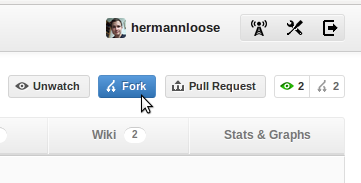
\includegraphics[width=12em]{fork}
    \end{column}
    \begin{column}{0.4\textwidth}
      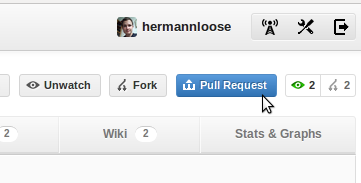
\includegraphics[width=12em]{pullrequest}
    \end{column}
  \end{columns}
  \begin{itemize}
    \item \texttt{https://github.com/hermannloose/escalator}
    \item \texttt{https://github.com/hermannloose/escalator-android}
  \end{itemize}
\end{frame}

\begin{frame}[c]
  \frametitle{Quellen}
  \begin{enumerate}
    \item http://guides.rubyonrails.org/ (Rails Guides)
    \item http://thoughtbot.com/community (Shoulda \& Factory Girl)
    \begin{itemize}
      \item https://github.com/thoughtbot/shoulda
      \item https://github.com/thoughtbot/factory\_girl
    \end{itemize}
    \item http://rspec.info/ (RSpec)
    \item http://developer.android.com/guide/index.html (Android Dev Guide)
  \end{enumerate}
\end{frame}

\end{document}
